\documentclass{spiral-kurs}
\def\title{Loch czarnoksiężnika}
\def\id{loc}
\def\TL{1~s}
\def\ML{256~MB}
\begin{document}
\makeheader
%

\begin{center}
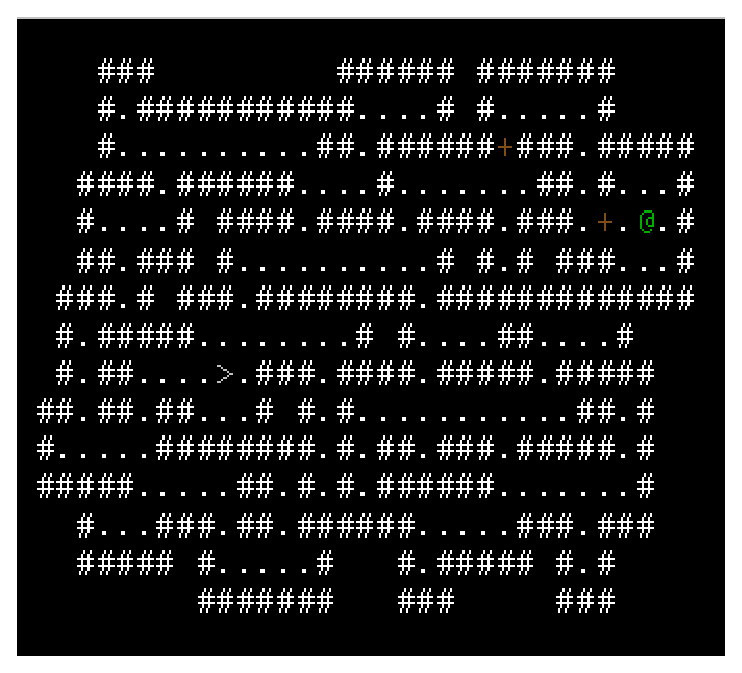
\includegraphics[width=0.5 \textwidth]{adom.eps}
\end{center}

  
Bohater (\texttt{@}) ucieka z lochu złego czarnoksiężnika. W jednym kroku może przejść o jedno pole na północ, południe, wschód lub zachód. Nie może, oczywiście, wejść na ścianę (\texttt{\#}), może jednak chodzić po wolnych polach (\texttt{.}) oraz przechodzić przez drzwi (\texttt{+}). 
Aby uciec, bohater musi stanąć na polu wyjściowym  (\texttt{>}). W jakiej najmniejszej liczbie kroków bohater może osiągnąć wyjście?

    \section{Wejście}

Pierwszy wiersz wejścia zawiera liczbę zestawów danych $Z$ -- dla każdego zestawu trzeba osobno obliczyć i podać odpowiedź. Kolejne wiersze zawierają opisy zestawów w następującej postaci:

W pierwszym wierszu zestawu znajdują się dwie liczby naturalne $m$, $n$ ($1 \leq m, n \leq 1000$) -- odpowiednio liczba wierszy i liczba kolumn planszy. W kolejnych $m$ wierszach znajduje się po $n$ znaków -- opis kolejnych wierszy planszy. Każdy znak jest jednym z wymienionych w opisie zadania. 
      
    \section{Wyjście}

Dla każdego zestawu wypisz \texttt{NIE}, jeśli ucieczka jest niemożliwa, lub jedną liczbę naturalną -- minimalną liczbę ruchów potrzebną do osiągnięcia wyjścia.


    \example{0}
  \end{document}
